% https://www.overleaf.com/learn/latex/LaTeX_Graphics_using_TikZ:_A_Tutorial_for_Beginners_(Part_1)%E2%80%94Basic_Drawing

\documentclass{article}

\usepackage{tikz}

\begin{document}
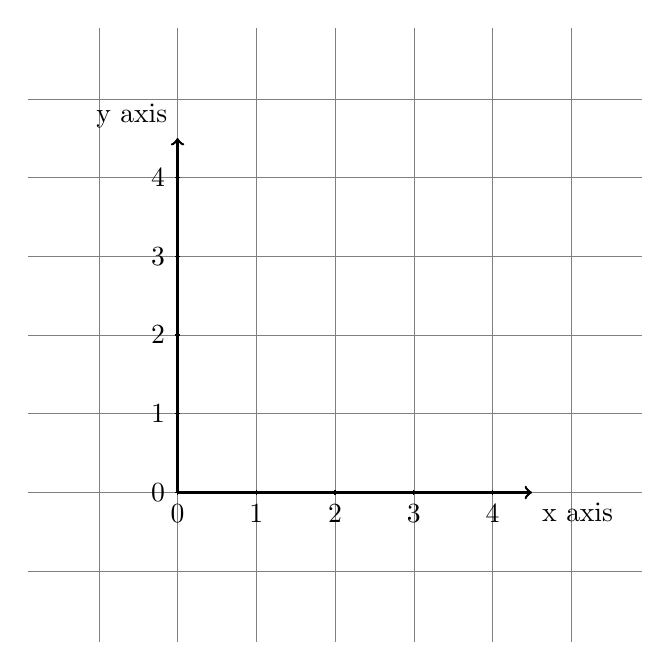
\begin{tikzpicture}
  % 点、线、矩形
  % \draw (0, 0) -- (4, 0);
  % \draw (0, 0) -- (4, 0) -- (4, 4) -- (0, 4) -- (0, 0);
  % \draw (0, 0) -- (4, 0) -- (4, 4) -- (0, 4) -- cycle;
  % \draw (0, 0) rectangle (4, 4);
 
  % 抛物线
  % \draw (0, 0) parabola (4, 4);
  % control points act like magnets attracting the line in their direction
  % \draw (0, 0) .. controls (0, 4) and (4, 0) .. (4, 4);
 
  % \draw (2, 2) circle (3cm);
  % 椭圆
  % \draw (2, 2) ellipse (3cm and 1cm);
  % 箭头:起始角、终止角、半径
  % \draw (3, 0) arc (0:180:3cm)

  % 自定义
  % \draw[red,thick,dashed] (2, 2) circle (3cm);

  % 网格
  % \draw[step=1cm,gray,very thin] (-2, -2) grid (6, 6)
  % 移去外边界
  \draw[step=1cm,gray,very thin] (-1.9, -1.9) grid (5.9, 5.9);
  % 在网格基础上进行颜色填充,40% 的蓝色,60% 的白色
  % \fill[blue!40!white] (0, 0) rectangle (4, 4);
  % 带边界的颜色填充
  % \filldraw[fill=blue!40!white, draw=black] (0,0) rectangle (4,4);
  % 从左至右渐变阴影
  % \shade[left color=blue,right color=red] (0,0) rectangle (4, 4);
  % 从上至下渐变阴影
  % \shade[top color=blue,bottom color=red] (0,0) rectangle (4, 4);
  % 由内而外渐变阴影
  % \shade[inner color=blue,outer color=red] (0,0) rectangle (4, 4);

  % 坐标
  % 带有 -> 的粗线
  \draw[thick,->] (0, 0) -- (4.5, 0);
  \draw[thick,->] (0, 0) -- (0, 4.5);
  % 加入坐标
  \draw[thick,->] (0, 0) -- (4.5, 0) node[anchor=north west] {x axis};
  \draw[thick,->] (0, 0) -- (0, 4.5) node[anchor=south east] {y axis};
  % 加入坐标值
  \foreach \x in {0, 1, 2, 3, 4}
    \draw (\x cm, 1pt) -- (\x cm, -1pt) node[anchor=north] {$\x$};
  \foreach \y in {0, 1, 2, 3, 4}
    \draw (1pt, \y cm) -- (-1pt, \y cm) node[anchor=east] {$\y$};

\end{tikzpicture}

\end{document}